\documentclass[xcolor=x11names,table]{beamer}
\usepackage{beamerthemeCambridgeUS}  % CambridgeUS theme
\usepackage{float}  % perfect fit graphic with command [H]
%\usepackage{tabularx}  % alternate to tabular to use X to wrap column data properly
%\usetheme{Antibes}
\usepackage{hyperref}

%package for timeline
\usepackage[utf8]{inputenc}
\usepackage[english]{babel}
\usepackage[TS1,T1]{fontenc}
\usepackage{fourier, heuristica}
\usepackage{array, booktabs}
%\usepackage[x11names]{xcolor}
%\usepackage{caption}
%\DeclareCaptionFont{blue}{\color{LightSteelBlue3}}

\newcommand{\foo}{\color{LightSteelBlue3}\makebox[0pt]{\textbullet}\hskip-0.5pt\vrule width 1pt\hspace{\labelsep}}



% for themes, etc.
%\mode<presentation>
%{ \usetheme{boxes} }

\usepackage{times}  % fonts
\usepackage{graphicx, wrapfig, caption} % for graphics
\usepackage{multirow}



%colours
\definecolor{lightblue}{rgb}{0.1, 0.1, 0.6}
\definecolor{maroon}{rgb}{0.3, 0.1, 0.7}

\newcommand{\FR}[2]{
	{\textstyle \frac{#1}{#2} }}
\def\RR{\mathbb{R}}



% macros
\newcommand{\hhq}{{\scriptstyle{{\frac{1}{4}}}}}
\newcommand\hf{\textstyle{1\over 2 }\displaystyle}
\newcommand\hhf{\scriptstyle{1\over 2 }\displaystyle}
\newcommand{\erf}{\mathrm{erf}}
\def\h{\textcolor{red}{\mathbf{h}}}
\def\z{\textcolor{maroon}{\mathbf{z}}}
\newcommand{\zave}{\z_{\mathrm{ave}}}
\def\by{\textcolor{lightblue}{\mathbf{y}}}
\def\bv{\textcolor{blue}{\mathbf{v}}}
\def\bx{\textcolor{red}{\mathbf{x}}}
\def\bp{\textcolor{maroon}{\mathbf{p}}}
\makeatother
\setbeamertemplate{footline}
{
	\leavevmode%
	\hbox{%
		\begin{beamercolorbox}[wd=.4\paperwidth,ht=2.25ex,dp=1ex,center]{author in head/foot}%
			\usebeamerfont{author in head/foot}\insertshortauthor
		\end{beamercolorbox}%
		\begin{beamercolorbox}[wd=.6\paperwidth,ht=2.25ex,dp=1ex,center]{title in head/foot}%
			\usebeamerfont{title in head/foot}\insertshorttitle\hspace*{3em}
			%			\insertframenumber{} / \inserttotalframenumber\hspace*{1ex}
	\end{beamercolorbox}}%
	\vskip0pt%
}
\makeatletter
\setbeamertemplate{navigation symbols}{}




% these will be used later in the title page
\title{Multi-programming}
\subtitle{An overview on Parallel Processing with Silicon, Graphics and Quantum Chips}
\author{Gahan Saraiya}
\institute{Firmware Development Engineer 
	\\ Intel Technology India Pvt Ltd}
\date{{\scriptsize March 2023}}

% note: do NOT include a \maketitle line; also note that this title
% material goes BEFORE the \begin{document}
	
% Recurring Outline for every section, with highlighting
\AtBeginSection[]
{ \begin{frame}<beamer> 
		\frametitle{Outline of Talk}
		\tableofcontents[currentsection]%[pausesections]
\end{frame} }
	
\begin{document}
	
	\begin{frame}
		\titlepage
	\end{frame}
	
	
	\section{Introduction}
	
	
	\begin{frame}[allowframebreaks]
		\frametitle{Overview of Coverage}
		\begin{itemize}
			\item Basics of Parallel Processing
			{\scriptsize \\ Multi-programming, Multi-core Programming}
			\item Computing Core Types
				{\scriptsize 
					\\ CPU - Central Processing Unit
					\\ GPU - Graphics Processing Unit
					\\ QPU - Quantum Processing Unit
				}
			\item Complexity of Solution
				{\scriptsize
					\\ Complexity of implementation with CPU, GPU, QPU
				}
			\item Scalability of Architecture
		\end{itemize}
		%\vspace{1cm}
	\end{frame}
	
	\section{Basics of Parallel Processing}
	\begin{frame}
		\frametitle{Types of parallel processing}
		\begin{itemize}
			\item Single Instruction, Single Data (SISD)
			\item Multiple Instruction, Single Data (MISD)
			\item Single Instruction, Multiple Data (SIMD)
			\item Multiple Instruction, Multiple Data (MIMD)
			\item Single Program, Multiple Data (SPMD)
			\item Massively Parallel Processing (MPP)
		\end{itemize}
		%\vspace{1cm}
	\end{frame}
	
	\section{Compute Architectures}
	\begin{frame}
		\frametitle{CPU - Central Processing Unit}
		\begin{figure}[p]
%			\caption{Reference: https://www.researchgate.net/figure/High-level-architecture-of-modern-processors_fig7_323941692}
			\centering
			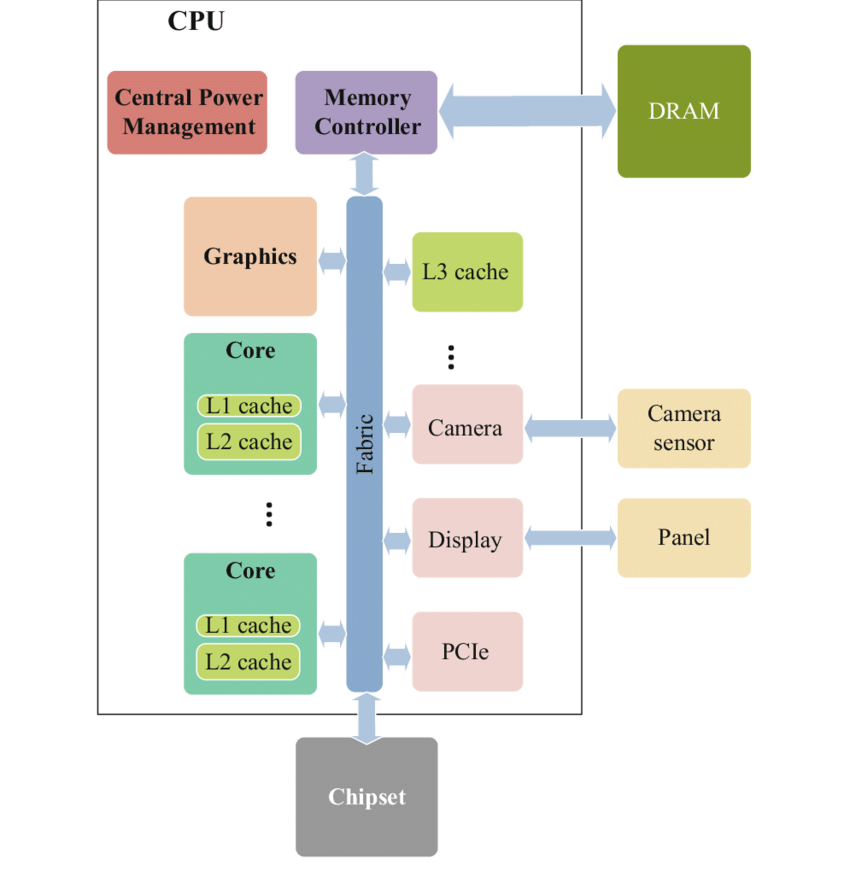
\includegraphics[width=\linewidth,height=\dimexpr\textheight-2\baselineskip-\abovecaptionskip-\belowcaptionskip\relax,keepaspectratio]{refs/High-level-architecture-of-modern-processors.png}
			\label{fig:cpu-architecture}
		\end{figure}
	
		%\vspace{1cm}
	\end{frame}
	
	\begin{frame}[allowframebreaks]
		\frametitle{GPU - Graphics Processing Unit}
		\begin{figure}[!h]
			\centering
			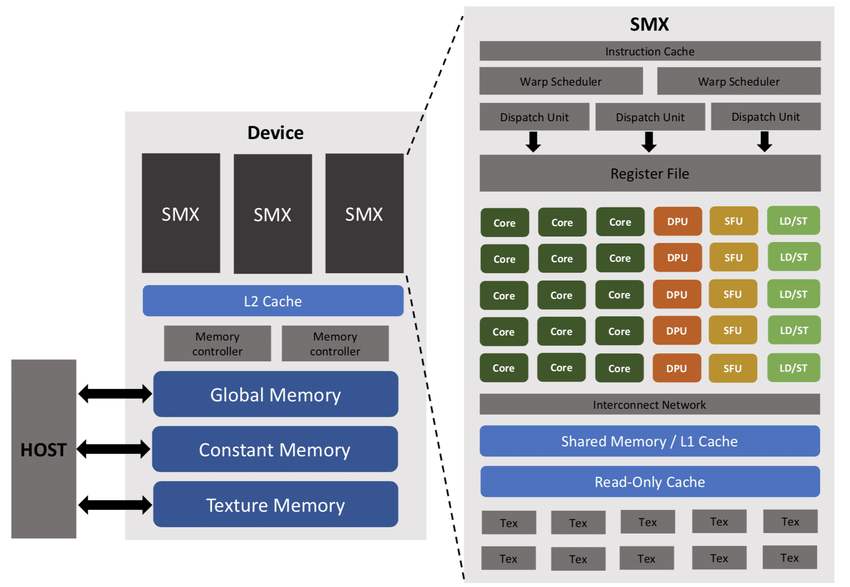
\includegraphics[width=\linewidth,height=\dimexpr\textheight-2\baselineskip-\abovecaptionskip-\belowcaptionskip\relax,keepaspectratio]{refs/Typical-NVIDIA-GPU-architecture-The-number-of-SMXs-and-the-computation-resources-inside.png}
			\label{fig:gpu-architecture}
		\end{figure}
	
		\begin{figure}[!h]
			\centering
			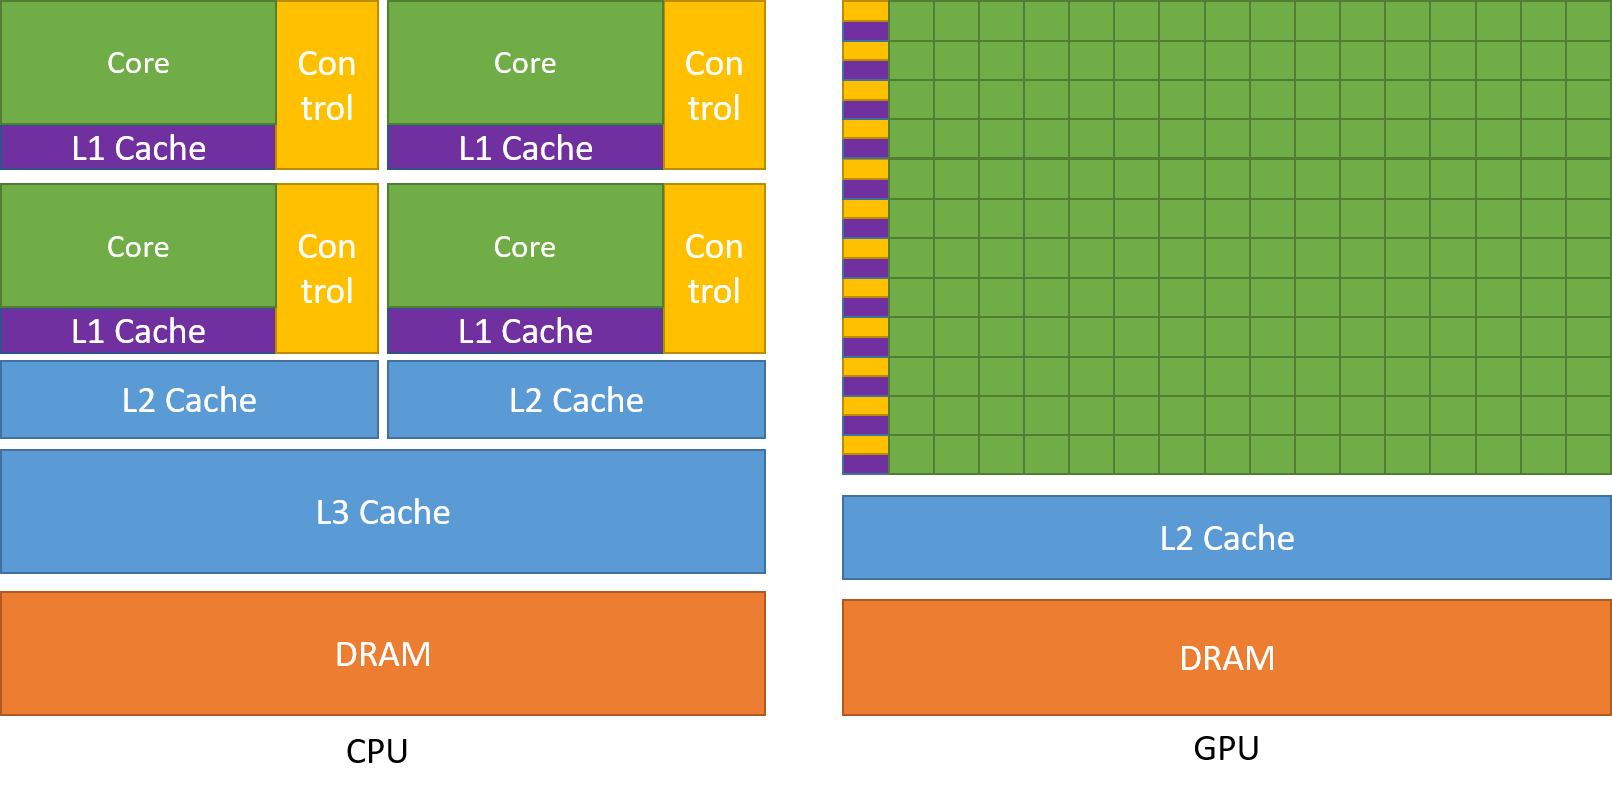
\includegraphics[width=\linewidth,height=\dimexpr\textheight-2\baselineskip-\abovecaptionskip-\belowcaptionskip\relax,keepaspectratio]{refs/gpu-devotes-more-transistors-to-data-processing.png}
			\label{fig:cpu-gpu-architecture}
		\end{figure}
	
	    \begin{tabular}{|c|c|c|} \hline
				Parameter & CPU & GPU  \\ \hline
				interviewer
		\end{tabular}
	\end{frame}

	\begin{frame}{|c||l||r|}
		\frametitle{QPU - Quantum Processing Unit}
		\begin{figure}[p]
			\centering
			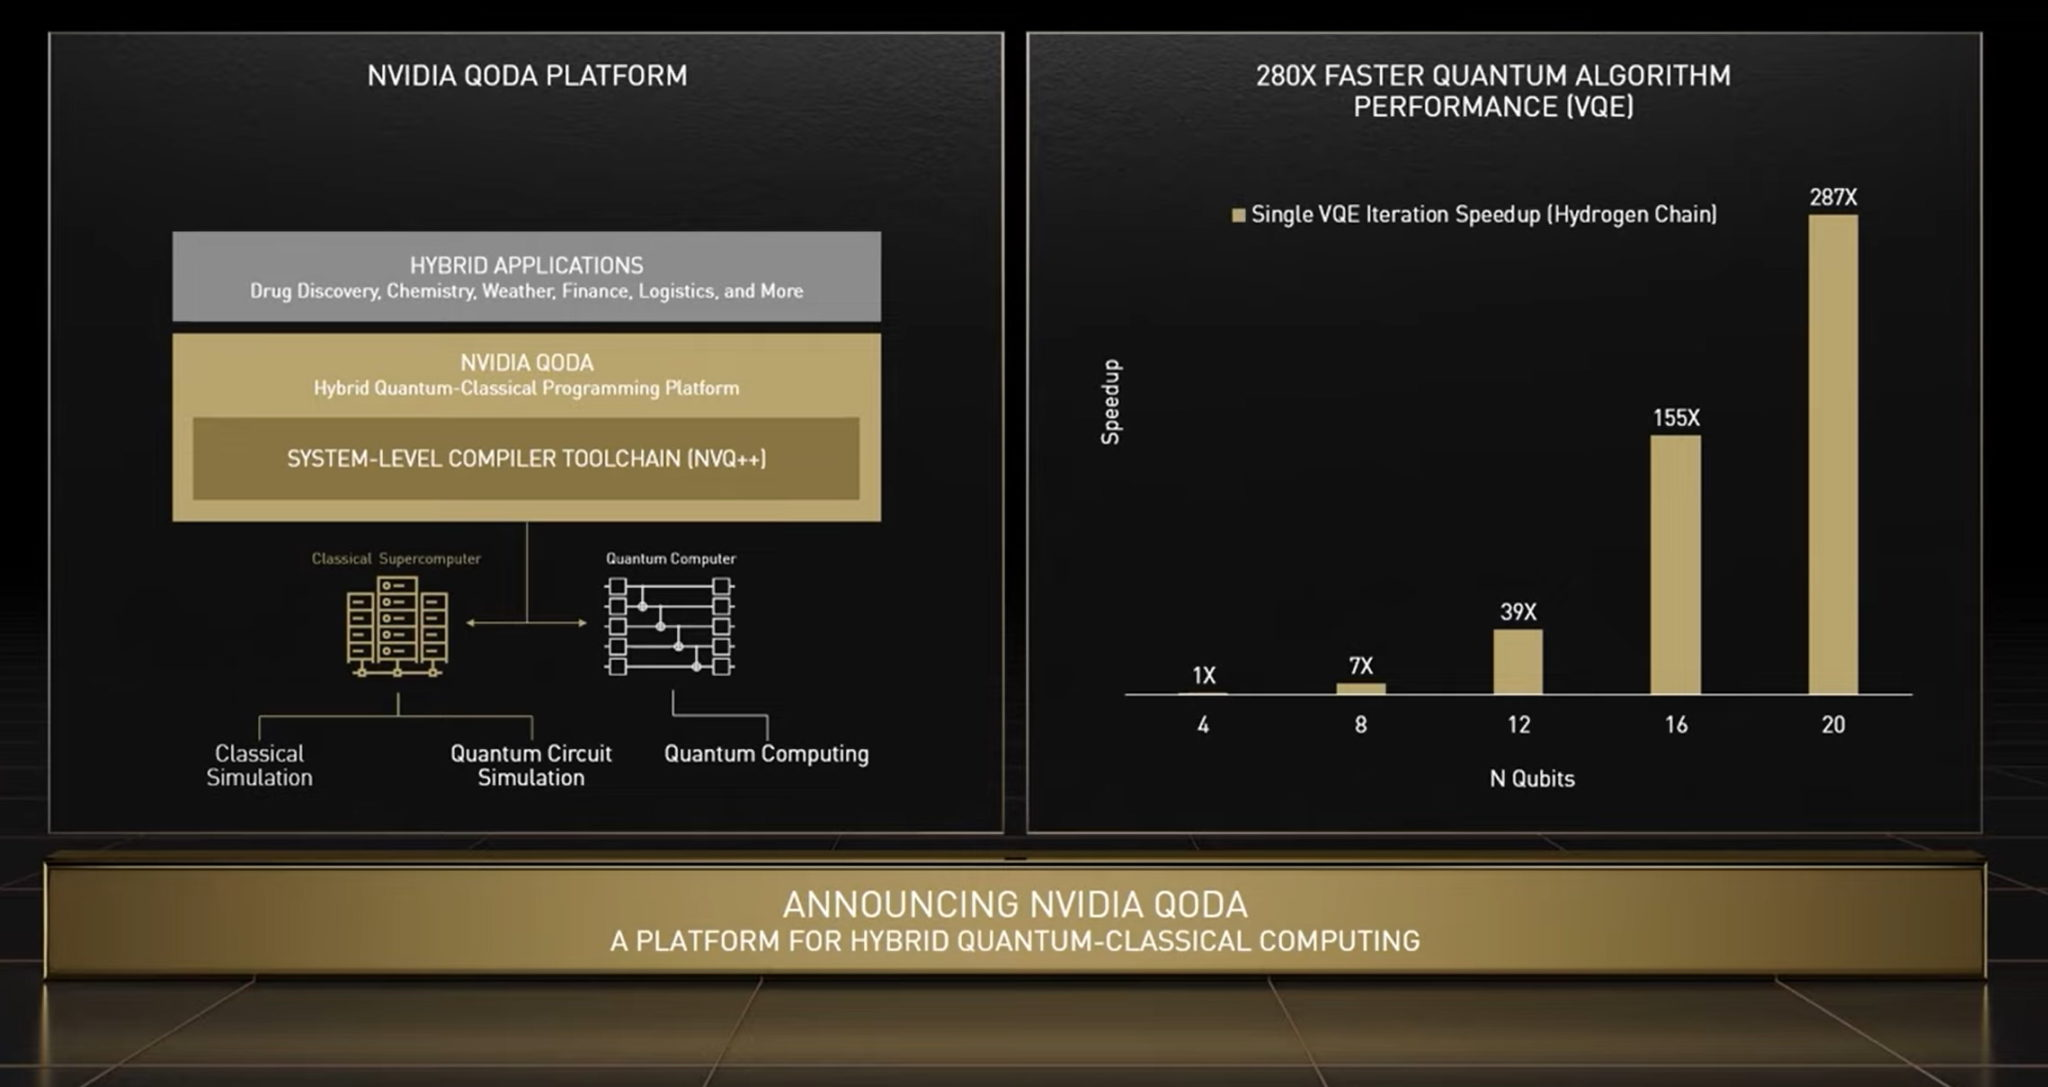
\includegraphics[width=\linewidth,height=\dimexpr\textheight-2\baselineskip-\abovecaptionskip-\belowcaptionskip\relax,keepaspectratio]{refs/QODA-slide-BEST-scaled.jpg}
			\label{fig:qpu-architecture-nvidia-qoda}
		\end{figure}
	\end{frame}
	
	\section{Quantum Architecture}
	
	\begin{frame}[allowframebreaks]
		\frametitle{Applications}
		\begin{itemize}
			\item \textbf{Optimization}
			\begin{itemize}
				\item systems design
				\item airline scheduling
				\item mission planning
				\item financial analysis
				\item web search
				\item cancer radiotherapy
				\item Volkswagen was the first car manufacturer to use a quantum computer to calculate traffic flows. 
				\item Recruit Communications and D-Wave - collaborated to apply quantum computing to marketing, advertising and communications. (optimize the efficiency of matching advertisements to customers for web advertising.)
			\end{itemize}
			\newpage
			
			\item \textbf{Machine Learning}
			\begin{itemize}
				\item Improving forecast capability with neural network
				\item learn to recognize essences of objects by recognizing patterns in huge amount of data
				\item native capability of D-Wave Quantum Processing Unit (QPU)
				\item NASA scientists trained the D-Wave 2X system on image data sets in a generative unsupervised learning 
			\end{itemize}
			\newpage
			
			\item \textbf{Biomedical Simulations}
			\begin{itemize}
				\item simulate molecular structures
				\item Using D-wave One quantum computer researchers from Harvard University solved the puzzle of how some proteins fold in year 2012 
			\end{itemize}
			
			\item \textbf{Financial Services}
			\begin{itemize}
				\item complex financial modeling and risk management within the financial industry
				\item new ways to model financial data
				\item isolate primary global risk factors
			\end{itemize}
		\end{itemize}
	\end{frame}
	
	\begin{frame}[allowframebreaks]
		\frametitle{Top Quantum Computing Companies}
		\begin{itemize}
			\item \href{https://www.dwavesys.com/}{D-wave Systems}
			\\ {\scriptsize
				World's first Quantum Computing Company
				\\ integrates new discoveries in physics, engineering, manufacturing and computer science into computational breakthrough approaches to solve most complex challenges.
			}
			\item IBM Quantum Computing
			\\ {\scriptsize Offers \href{https://quantumexperience.ng.bluemix.net/}{quantum experience} on cloud-enabled quantum computing platform
				\\ allows user to run algorithms, experiments, work on qubits, simulation etc.}
			\item Microsoft Quantum Computing
			\\ {\scriptsize Conducts theoretical and experimental approaches to creating quantum computers}
			\item Google Research
			\\ {\scriptsize
				Quantum Artificial Intelligence Lab - joint initiative of NASA, Universities Space Research Association and Google Research
				\\ goal - how quantum computing help with machine learning and other complex problems of computer science
				\\ Lab hosted at NASA's Ames Research Center
			}
			\item \href{www.toshiba.eu/eu/Cambridge-Research-Laboratory/Quantum-Information-Group/}{Toshiba Quantum Information Group}
			\\ {\scriptsize
				Research teams on Quantum Information, Speech Technology and Computer Vision.
				\\ Collaboration with Cavendish Laboratory and Engineering Department of the University, Cambridge and Toshiba R\&D groups.
			}
			\item \href{https://newsroom.intel.com/tag/qutech/}{Intel}
			\\ {\scriptsize 
				10 year collaboration with institute \href{https://qutech.nl/qutechentersintocollaborationwithintel/}{QuTech}, Netherlands formed in 2013 by Delft University of Technology for Applied Research in Quantum Computers
			}
			\item Alibaba Quantum Computing Laboratory
			\\ {\scriptsize
				goal - bring study and applications to the next level, platform for connectivity, computing and information security
			}
			\item Cambridge Quantum Computing
			\\ {\scriptsize
				independent company - expertise in Quantum Information Processing, AI, Optimization and pattern recognition
			}
			\item And many more...
			\\ {\scriptsize
				HP Lab : Quantum Information Processing, 1QB Information Technologies, Lockheed Martin, Regetti, IONQ, QxBranch, Post-Quantum, ID Quantique, QuintessenceLabs, Quantum Biosystems
			}
		\end{itemize}
	\end{frame}
	
	\begin{frame}
		\frametitle{Types of Quantum Processor}
		\begin{block}{\textbf{Silicon Spin Qubits}}
			Electrons or nuclear spins on a solid subtract
		\end{block}
		\begin{block}{\textbf{Superconducting Circuits}}
			currents superposition around superconductor
		\end{block}
		\begin{block}{\textbf{Ion's Trap}}
			Trap ions in electric fields
		\end{block}
		\begin{block}{\textbf{Photonic Circuits}}
			qubits are photons driven in silicon circuits
		\end{block}
	\end{frame}
	
	\begin{frame}
		\frametitle{Timeline}
		\begin{table}
			\renewcommand\arraystretch{1.1}\arrayrulecolor{LightSteelBlue3}
			%		\captionsetup{singlelinecheck=false, font=blue, labelfont=sc, labelsep=quad}
			%		\caption{Timeline}\vskip -1.5ex
			\begin{tabular}{@{\,}r <{\hskip 2pt} !{\foo} >{\raggedright\arraybackslash}p{5cm} l}
				%			\toprule
				%			\addlinespace[1.5ex]
				May, 2011 & D-Wave One (Ranier) & 128qb \\
				2013 & D-Wave Two & 512 qb \\
				2015 & D-Wave 2X & 1152 qb \\
				2016 & IBM Q Experience 5 & 5qb \\
				2017 & Google & 20 qb \\
				2017 & D-Wave 2000Q & 2000 qb \\
				May, 2017 & IBM Q 16 & 16 qb \\
				May, 2017 & IBM Q 17 & 17 qb \\
				October, 2017 & Intel 17-Qubit Superconducting Test Chip & 17 qb \\
				November, 2017 & IBM Q 20 & 20 qb \\
				2017 & Rigetti 19Q & 19 qb \\
				January 2018 & Intel Tangle Lake & 49 qb \\
				March 2018 & Google Bristlecone & 72 qb \\
			\end{tabular}
		\end{table}
	\end{frame}
	
	

	
	\begin{frame}[allowframebreaks]
		\frametitle{Google AI Quantum}
		\begin{block}{Superconducting qubit processors}
			Superconducting qubits with chip-based scalable architecture targeting two-qubit gate error < 0.5\%. Google's Bristlecone is newest 72-qubit quantum processor\footnote{as on 2018}.
		\end{block}
		\begin{block}{Qubit metrology}
			Reducing two-qubit loss below 0.2\% is critical for error correction.
			\\ Working on a quantum supremacy experiment, to approximately sample a quantum circuit beyond the capabilities of state-of-the-art classical computers and algorithms.
		\end{block}
		\begin{block}{Quantum simulation}
			Simulation of physical systems is among the most anticipated applications of quantum computing.
			\\ quantum algorithms for modelling systems of interacting electrons with applications in chemistry and materials science.
		\end{block}
		\begin{block}{Quantum neural networks}
			a framework to implement a quantum neural network on near-term processors.
			\\ understanding advantages may arise from generate massive superposition states during operation of the network.
		\end{block}
		\begin{block}{Quantum assisted optimization}
			Developing hybrid quantum-classical solvers for approximate optimization.
			\\ Thermal jumps in classical algorithms to overcome energy barriers could be enhanced by invoking quantum updates.
			\\ Particular interested in coherent population transfer.
		\end{block}
	\end{frame}
	
	%	\begin{table}[H]
		%	\centering
		%		\begin{tabularx}{\linewidth}{ r X }
			%			\textbf{Silicon Spin Qubits}
			%			& 
			%			Electrons or nuclear spins on a solid subtract
			%			\\ 
			%			\textbf{Superconducting Circuits}
			%			& 
			%			currents superposition around superconductor
			%			\\ 
			%			\textbf{Ion's Trap}
			%			& 
			%			Trap ions in electric fields
			%			\\
			%			\textbf{Photonic Circuits}
			%			&
			%			qubits are photons driven in silicon circuits
			%		\end{tabularx}
		%	\end{table}
	
	
\end{document}
